%--------------------------------------------------
% Abstract
%-------------------------------------------------- 
\begin{abstract}
\comment{ 
  Abstract goes here...
  Abstract goes here...
  Abstract goes here...
  Abstract goes here...
}
\end{abstract}

%--------------------------------------------------
% Introduction
%-------------------------------------------------- 
\section{Introduction} \label{s:introduction}

Topic models, such as probabilistic latent-semantic analysis
\cite{hofmann1999probabilistic} and latent-Dirichlet allocation
\cite{blei2003latent}, were first introduced in the NLP community as a means of
formalizing the latent semantics from the surface data.  A large body of
research has made use of such techniques and benefit from all kinds of
successful implications branched from the original model.  Generally, most of
these previous efforts began with the assumption that a document is, in
principle, a bag of topics, and words that are observed were indirectly
inferred by the underlying distribution of these background topics.  The
process to go from a pseudo (or {\it prototypical}) document, composed of
latent semantics, to a realization of the document, i.e., collection of words,
is described as a generative statistical process that relies on two discrete
distributions: the document-level topic distribution $\Pr(z|d)$ and the
topic-specific word distribution $\Pr(w|z)$.  Such an arrangement has garnered
great success in various document-specific tasks.  However, direct implication
of such models on sentence data may cause problems due to the misjudgment of
the text boundaries.  

When applied on short text units without specific arrangement, the LDA model
either overfits the data or does not get good probabilistic estimate at all.
Usually we either end up modeling sentences the way we do with documents (as if
the sentences were smaller topics containers) and deliberately omit the
document-level information, or we completely ignore the sentence structures and
go with the original settings.  Either way we lose a certain amount of rich
information embedded in the sentence structure.  We find it cumbersome for
topic models being restricted to the implication on only one level of
granularity; Since a number of NLP applications might lean on any kind of
adaptation of LDA to model the sentence-word or document-sentence relationship,
we look for a way to mitigate the forementioned problems.

This work is motivated by the following hypothesis.  We assume that the
overfitting problem can be mitigate by by introducing a set of sentence-level
ensembles into the original LDA model.  The ensembles are indicators that point
to a set of multinomial distributions over topics; each sentence in the
document choose a distribution to follow and generates the word topics
accordingly.  The idea is to offer a \emph{switch} in between documents and
topics, serving as a soft boundary between short texts (as opposed to the usual
\emph{hard} boundary between sentences) that prevents the LDA model either go
low on the co-occurrence counts or grow overfitted.  

Our contribution can be stated as follows.  We proposed an adaptation for the
original LDA model to the sentence data; in the experiment our approach showed
better interpretability on the test benchmark, indicating that the adaptation
generalized well for sentences than original LDA model did. 

This paper is arranged as follows.  In Section~\ref{s:sentence-layered-lda}, we
introduce an LDA-based generative model to leverage the intra-document sentence
topics and the corresponding inference procedure.  The estimation method for
model parameters are describe in Section~\ref{s:parameter-estimation}.  The
experiments and results are shown in Section~\ref{s:perplexity-evaluation}.  Related work
is introduced in Section~\ref{s:related-work}.  In Section~\ref{s:discussions},
we discuss a number of interesting issues discovered in the development of the
work and give out conclusions.

%--------------------------------------------------
% Model
%-------------------------------------------------- 
\section{Sentence-Layered LDA} \label{s:sentence-layered-lda} We propose an
generative topic model called {\it sentence-layered LDA}, by biasing the
original latent-Dirichlet allocation framework toward an adapation {for} the
sentence structure.  We introduce the notion of {\it sentence topics} by adding
a set of latent variables in between the document and the words; the sentence
topics served as an additional sub-document layer that is responsible for
generating word topics.  We model the sentence topics as scalars, which in turn
refers to a discrete distribution over word topics.  The complete generative
process is depicted as follows.
\begin{table}[!ht]
  \footnotesize
  \centering
  \begin{tabular}{c}
    $\theta^{d} \sim \mathrm{Dirichlet}(\alpha)$ \\
    $x_j \sim \mathrm{Multinomial}(\theta^{(d)})$ \\
    $z_i \sim \mathrm{Discrete}(\tau^{(x_j)})$ \\
    $w_i \sim \mathrm{Discrete}(\phi^{(z_i)})$ \\
    $\tau^{(x_j)} \sim \mathrm{Dirichlet}(\gamma)$ \\
    $\phi^{(z_i)} \sim \mathrm{Dirichlet}(\beta)$ 
  \end{tabular}
\end{table}

%--------------------------------------------------
% \begin{eqnarray*}
%   \theta^{d} &\sim& \mathrm{Dirichlet}(\alpha) \\
%   x_j &\sim& \mathrm{Multinomial}(\theta^{(d)}) \\
%   z_i &\sim& \mathrm{Discrete}(\tau^{(x_j)}) \\
%   w_i &\sim& \mathrm{Discrete}(\phi^{(z_i)}) \\
%   \tau^{(x_j)} &\sim& \mathrm{Dirichlet}(\gamma) \\
%   \phi^{(z_i)} &\sim& \mathrm{Dirichlet}(\beta) 
% \end{eqnarray*}
%-------------------------------------------------- 

%--------------------------------------------------
% For each document $d$, we draw a multinomial distribution $\theta^{(d)}$ over
% sentence topics from the Dirichlet prior $\alpha$.  Then, we draw a number of
% sentence topics $x_j$ from $\theta^{(d)}$ for all the sentences in the
% document.  Each sentence topic $x_j$ then leads to a discrete distribution over
% word topics, which is denoted as $\tau^{(x_j)}$, that we could use to draw word
% topics from.  Let each word topic drawn from $\tau^{(x_j)}$ be denoted as
% $z_i$, which again leads to a discrete distribution $\phi^{(z_i)}$ over words.
% Finally, we draw a word $w_i$ from the distribution $\phi^{(z_i)}$ for each
% word in the sentence.  
%-------------------------------------------------- 
As a general assumption of the model, all the
discrete distributions $\tau^{(x_j)}$ were governed by the Dirichlet prior
$\gamma$ and all the discrete distributions $\phi^{(z_i)}$ by the Dirichlet
prior $\beta$.  The plate notation is shown in
Figure~\ref{plate-notation:sentence-layered}.

\begin{figure}[ht!]
  \centering
  \psset{xunit=7mm,yunit=7mm}
  \begin{pspicture}(0,0)(8,11)%\showgrid  % Uncomment to show grid!
    \SpecialCoor  % (a|b) means x-coord from 'a' and y-coord from 'b'.
    \psset{arrowscale=1.5}

    \rput(2.0,10.0){\GM@parameter{alpha}}\GM@label[angle=45]{alpha}{$\alpha$}
    \rput(alpha|0,8.0){\GM@node{theta}}\GM@label[angle=45]{theta}{$\theta$}
    \rput(alpha|0,6.0){\GM@node{x}}\GM@label[angle=45]{x}{$x$}
    \rput(alpha|0,4.0){\GM@node{z}}\GM@label[angle=45]{z}{$z$}
    \rput(alpha|0,2.0){\GM@node[observed=true]{w}}\GM@label[angle=45]{w}{$w$}
    \rput(1.25,1.25){\GM@plate{1.5}{3.5}{$N_x$}}
    \rput(0.75,0.75){\GM@plate{2.5}{6.0}{$M_\theta$}}
    \rput(0.25,0.25){\GM@plate{3.5}{8.5}{$L$}}
    
    \rput(7.0,0|w){\GM@parameter{beta}}\GM@label[angle=45]{beta}{$\beta$}
    \rput(7.0,0|z){\GM@parameter{delta}}\GM@label[angle=45]{delta}{$\delta$}
    \rput(5.0,0|w){\GM@node{phi}}\GM@label[angle=45]{phi}{$\phi$}
    \rput(5.0,0|z){\GM@node{tau}}\GM@label[angle=45]{tau}{$\tau$}
    \rput(4.25,3.25){\GM@plate{1.5}{1.5}{$S$}}
    \rput(4.25,1.25){\GM@plate{1.5}{1.5}{$T$}}

    \ncline[arrows=->]{alpha}{theta}
    \ncline[arrows=->]{theta}{x}
    \ncline[arrows=->]{x}{z}
    \ncline[arrows=->]{z}{w}
    \ncline[arrows=->]{beta}{phi}
    \ncline[arrows=->]{delta}{tau}
    \ncline[arrows=->]{tau}{z}
    \ncline[arrows=->]{phi}{w}
  \end{pspicture}
  \caption{The sentence-layered LDA model in the plate notation}
  \label{plate-notation:sentence-layered}
\end{figure}

We apply a Gibbs sampler to induce the model.  Since the joint probability
$\Pr(\mathbf{z}, \mathbf{x})$ is generally intractable, we break it down to
several conditional probability distributions.  The derivation largely follows
the paradigm established in \cite{blei2003latent} and
\cite{griffiths2004finding}, making use of conjugate priors to simplify the
inference.

\paragraph{Conditional for $\mathbf{z_i}$.}  The conditional distribution $\Pr(z_i
= j|\mathbf{z}_{-i}, \mathbf{w}, \mathbf{x})$ can be derived as what follows.
\begin{small}
\begin{eqnarray*}
  && \Pr(z_i = j|\mathbf{z}_{-i}, \mathbf{w}, \mathbf{x}) \nonumber\\
  && \propto \Pr(w_i|z_i = j, \mathbf{z}_{-i}, \mathbf{w}_{-i}) \Pr(z_i = j|\mathbf{z}_{-i}, x, \mathbf{x}') \nonumber \\
  && = \frac{\beta + n_{-i,j}^{(w_i)}}{V \beta + n_{-i,j}^{(\cdot)}} \frac{\delta + n_{-i,x}^{(j)}}{T \delta + n_{-i,x}^{(\cdot)}}, \label{z_i:2.3}
\end{eqnarray*}
\end{small}

Here, $x$ denotes the sentence topic that induces $z_i$, and $\mathbf{x}' =
\mathbf{x} - \{ x \}$.  $n_{-i,j}^{(\cdot)}$ denotes the counts for all word
occurrences that are of word topic $j$, excluding the current assignment of
$w_i$, which is defined by $n_{-i,j}^{(\cdot)} = \sum_w n_{-i,j}^{(w)}$.  In a
similar way, $n_j^{(\cdot)}$ denotes all such assignments including the count
for $w_i$, which is defined by $n_j^{(\cdot)} = \sum_w n_j^{(w)}$.  lso note
  that $n_j^{(w_i)} = n_{-i,j}^{(w_i)} + 1$ and $n_j^{(w)} = n_{-i,j}^{(w)}$
  for all $w \ne w_i$.

%--------------------------------------------------
% \begin{eqnarray}
%     && \Pr(z_i = j|\mathbf{z}_{-i}, \mathbf{w}, \mathbf{x}) \nonumber\\
%     &=& \Pr(z_i = j|\mathbf{z}_{-i}, w_i, \mathbf{w}_{-i}, x, \mathbf{x}') \nonumber\\
%     &\propto& \Pr(w_i|z_i = j, \mathbf{z}_{-i}, \mathbf{w}_{-i}) \nonumber\\
%     && \times \Pr(z_i = j|\mathbf{z}_{-i}, x, \mathbf{x}') \label{z_i:both},
% \end{eqnarray}
%-------------------------------------------------- 

%--------------------------------------------------
% The first term in \eqref{z_i:both} is expanded by introducing the random variable $\phi^{(j)}$.
% Appropriate invocation of Bayes' theorem over the first term lead us to the simplified form.
% \begin{eqnarray}
%   && \Pr(w_i|z_i = j, \mathbf{z}_{-i}, \mathbf{w}_{-i}) \nonumber \\
%   && = \int \Pr(w_i|\phi^{(j)},z_i = j,\mathbf{z}_{-i},\mathbf{w}_{-i}) \nonumber\\
%   && \quad \Pr(\phi^{(j)}|z_i = j,\mathbf{z}_{-i},\mathbf{w}_{-i})\mathrm{d}\phi^{(j)} \nonumber \\
%   && = \frac{\beta + n_{-i,j}^{(w_i)}}{V \beta + n_{-i,j}^{(\cdot)}} \int \frac{\Gamma(V \beta + n_j^{(\cdot)})}{\prod_w \Gamma(\beta + n_j^{(w)})} \nonumber\\
%   && \quad \prod_w \left(\phi^{(j)}_w\right)^{\beta + n_j^{(w)} - 1} \mathrm{d}\phi^{(j)} \label{z_i:1.2} \\
%   && = \frac{\beta + n_{-i,j}^{(w_i)}}{V \beta + n_{-i,j}^{(\cdot)}}, \label{z_i:1.3}
% \end{eqnarray}
% 
% Here, $n_{-i,j}^{(\cdot)}$ denotes the counts for all word occurrences that are
% of word topic $j$, excluding the current assignment of $w_i$, defined by
% $n_{-i,j}^{(\cdot)} = \sum_w n_{-i,j}^{(w)}$.  In a similar way,
% $n_j^{(\cdot)}$ denotes all such assignments including the count for $w_i$,
% which is defined by $n_j^{(\cdot)} = \sum_w n_j^{(w)}$.  The derivation largely
% follows the paradigm established in \cite{blei2003latent} and \cite{griffiths2004finding}, making
% use of conjugate priors to simplify the inference.  By employing the property
% $\Gamma(k + 1) = k \Gamma(k)$, we are able to further reduce the equation to
% the form of \eqref{z_i:1.2} and \eqref{z_i:1.3}.  Also note that $n_j^{(w_i)} =
% n_{-i,j}^{(w_i)} + 1$ and $n_j^{(w)} = n_{-i,j}^{(w)}$ for all $w \ne w_i$.
% 
% The second term of \eqref{z_i:both} is also dealt with in the similar way. We expanded and intergrated the term over $\tau^{(x)}$ and it led us to the following derivation.
% \begin{eqnarray}
%   && \Pr(z_i = j|\mathbf{z}_{-i}, x, \mathbf{x}') \nonumber \\
%   && = \int \Pr(z_i = j|\tau^{(x)}, \mathbf{z}_{-i}, x, \mathbf{x}') \nonumber\\
%   && \quad \Pr(\tau^{(x)}|\mathbf{z}_{-i}, x, \mathbf{x}')\mathrm{d}\tau^{(x)} \nonumber \\
%   && = \int \tau_j^{(x)} \frac{\Gamma(T \delta + n_{-i,x}^{(\cdot)})}{\prod_z \Gamma(\delta + n_{-i,x}^{(z)})} \nonumber\\
%   && \quad \prod_z \left(\tau^{(x)}_z\right)^{\delta + n_{-i,x}^{(z)} - 1} \mathrm{d}\tau^{(x)} \label{z_i:2.1} \\
%   && = \frac{\delta + n_{-i,x}^{(j)}}{T \delta + n_{-i,x}^{(\cdot)}} \int \frac{\Gamma(T \delta + n_x^{(\cdot)})}{\prod_z \Gamma(\delta + n_x^{(z)})} \nonumber\\
%   && \quad \prod_z \left(\tau^{(x)}_z\right)^{\delta + n_x^{(z)} - 1} \mathrm{d}\tau^{(x)} \label{z_i:2.2} \\
%   && = \frac{\delta + n_{-i,x}^{(j)}}{T \delta + n_{-i,x}^{(\cdot)}}, \label{z_i:2.3}
% \end{eqnarray}
% where $n_{-i,x}^{(j)}$ denotes the number of words being assigned to topic $j$
% that are also governed by sentences assigned to the same topic as that of $x$,
% with the current word ($w_i$) left out.  In other words, we consider only
% sentences that are of same sentence-level topic as that of $x$ and count the
% number of words in these sentences being assigned to topic $j$.  Note that
% $n_x^{(j)} = n_{-i,x}^{(j)} + 1$ and $n_x^{(z)} = n_{-i,x}^{(z)}$ for all $z \ne
% z_i$.   Equation \eqref{z_i:2.1} follows the fact that
% $\Pr(\tau^{(x)}|\mathbf{z}_{-i}, x, \mathbf{x}') \propto \Pr(\mathbf{z}_{-i}|x,
% \mathbf{x}', \tau^{(x)}) \Pr(\tau^{(x)}) \sim \mathrm{Dirichlet}(\delta +
% n_{-i,x}^{(z)})$, and equations \eqref{z_i:2.2} and \eqref{z_i:2.3} from the
% same rationale as what we have in the preceding paragraph.
%-------------------------------------------------- 
%--------------------------------------------------
% \begin{eqnarray}
%   && \Pr(w_i|z_i = j, \mathbf{z}_{-i}, \mathbf{w}_{-i}) \nonumber \\
%   &=& \int \Pr(w_i|\phi^{(j)},z_i = j,\mathbf{z}_{-i},\mathbf{w}_{-i}) 
%   \Pr(\phi^{(j)}|z_i = j,\mathbf{z}_{-i},\mathbf{w}_{-i})\mathrm{d}\phi^{(j)} \nonumber \\
%   &=& \int \Pr(w_i|\phi^{(j)},z_i = j) \Pr(\phi^{(j)}|\mathbf{z}_{-i},\mathbf{w}_{-i})\mathrm{d}\phi^{(j)} \nonumber \\
%   &=& \int \phi^{(j)}_{w_i} \frac{\Gamma(V \beta + n_{-i,j}^{(\cdot)})}{\prod_w \Gamma(\beta + n_{-i,j}^{(w)})} \prod_w \left(\phi^{(j)}_w\right)^{\beta + n_{-i,j}^{(w)} - 1} \mathrm{d}\phi^{(j)} \label{z_i:1.1} \\
%   &=& \frac{\beta + n_{-i,j}^{(w_i)}}{V \beta + n_{-i,j}^{(\cdot)}} \int \frac{\Gamma(V \beta + n_j^{(\cdot)})}{\prod_w \Gamma(\beta + n_j^{(w)})} \prod_w \left(\phi^{(j)}_w\right)^{\beta + n_j^{(w)} - 1} \mathrm{d}\phi^{(j)} \label{z_i:1.2} \\
%   &=& \frac{\beta + n_{-i,j}^{(w_i)}}{V \beta + n_{-i,j}^{(\cdot)}}, \label{z_i:1.3}
% \end{eqnarray}
% where $n_{-i,j}^{(\cdot)} = \sum_w n_{-i,j}^{(w)}$ and $n_j^{(\cdot)} = \sum_w n_j^{(w)}$.  Equation
% \eqref{z_i:1.1} follows the fact that
% $\Pr(\phi^{(j)}|\mathbf{z}_{-i},\mathbf{w}_{-i}) \propto
% \Pr(\mathbf{w}_{-1}|\mathbf{z}_{-1},\phi^{(j)}) \Pr(\phi^{(j)}) \sim
% \mathrm{Dirichlet}(\beta + n_{-i,j}^{(w)})$.  By employing the property $\Gamma(k + 1) = k
% \Gamma(k)$, we are able to further reduce the equation to the form of
% \eqref{z_i:1.2} and \eqref{z_i:1.3}.  Also note that $n_j^{(w_i)} = n_{-i,j}^{(w_i)} + 1$ and $n_j^{(w)} =
% n_{-i,j}^{(w)}$ for all $w \ne w_i$.
%-------------------------------------------------- 

%--------------------------------------------------
% In the same way, we have the second term of \eqref{z_i:both} expanded and intergrated over $\tau^{(x)}$.
% \begin{eqnarray}
%   && \Pr(z_i = j|\mathbf{z}_{-i}, x, \mathbf{x}') \nonumber \\
%   &=& \int \Pr(z_i = j|\tau^{(x)}, \mathbf{z}_{-i}, x, \mathbf{x}') 
%   \Pr(\tau^{(x)}|\mathbf{z}_{-i}, x, \mathbf{x}')\mathrm{d}\tau^{(x)} \nonumber \\
%   &=& \int \Pr(z_i = j|\tau^{(x)}, x) \Pr(\tau^{(x)}|\mathbf{z}_{-i}, x,\mathbf{x}')\mathrm{d}\tau^{(x)} \nonumber \\
%   &=& \int \tau_j^{(x)} \frac{\Gamma(T \delta + n_{-i,x}^{(\cdot)})}{\prod_z \Gamma(\delta + n_{-i,x}^{(z)})} \prod_z \left(\tau^{(x)}_z\right)^{\delta + n_{-i,x}^{(z)} - 1} \mathrm{d}\tau^{(x)} \label{z_i:2.1} \\
%   &=& \frac{\delta + n_{-i,x}^{(j)}}{T \delta + n_{-i,x}^{(\cdot)}} \int \frac{\Gamma(T \delta + n_x^{(\cdot)})}{\prod_z \Gamma(\delta + n_x^{(z)})} \prod_z \left(\tau^{(x)}_z\right)^{\delta + n_x^{(z)} - 1} \mathrm{d}\tau^{(x)} \label{z_i:2.2} \\
%   &=& \frac{\delta + n_{-i,x}^{(j)}}{T \delta + n_{-i,x}^{(\cdot)}}.  \label{z_i:2.3}
% \end{eqnarray}
% where $n_{-i,x}^{(j)}$ denotes the number of words being assigned to topic $j$
% that are also governed by sentences assigned to the same topic as that of $x$,
% with the current word ($w_i$) left out.  In other words, we consider only
% sentences that are of same sentence-level topic as that of $x$ and count the
% number of words in these sentences being assigned to topic $j$.  Note that
% $n_x^{(j)} = n_{-i,x}^{(j)} + 1$ and $n_x^{(z)} = n_{-i,x}^{(z)}$ for all $z \ne
% z_i$.   Equation \eqref{z_i:2.1} follows the fact that
% $\Pr(\tau^{(x)}|\mathbf{z}_{-i}, x, \mathbf{x}') \propto \Pr(\mathbf{z}_{-i}|x,
% \mathbf{x}', \tau^{(x)}) \Pr(\tau^{(x)}) \sim \mathrm{Dirichlet}(\delta +
% n_{-i,x}^{(z)})$, and equations \eqref{z_i:2.2} and \eqref{z_i:2.3} from the
% same rationale as what we have in the preceding paragraph.
%-------------------------------------------------- 

\paragraph{Conditional $x$.}  The conditional $\Pr(x =
l|\mathbf{x}',\mathbf{z})$ can be rewritten as: 
\begin{small}
\begin{eqnarray*}
  && \Pr(x = l|\mathbf{x}',\mathbf{z}) \nonumber\\
  && \propto \Pr(\mathbf{z}^*|x = l, \mathbf{x}', \mathbf{z}') \Pr(x = l |\mathbf{x}',\mathbf{z}') \\
  && = \frac{\mathcal{B}(\{\delta + n_l^{(z)}; \forall z\})}{\mathcal{B}(\{\delta + n_{-x,l}^{(z)}; \forall z\})}
  \frac{\alpha + n_{-x,d}^{(l)}}{S \alpha + n_{-x,d}^{(\cdot)}}.
\end{eqnarray*}
\end{small}
where $\mathbf{x}' =
\mathbf{x} - \{x\}$, $\mathbf{z}^*$ and $\mathbf{z}'$ denotes all the topics
governed by the current sentence and the others, respectively (i.e.,
$\mathbf{z} = \mathbf{z}^* \cup \mathbf{z}'$).
Note that $\mathcal{B}(\cdot)$ is the multinomial beta function defined by
\[\mathcal{B}(a_1, \ldots, a_n) = \frac{\prod_i \Gamma(a_i)}{\Gamma(\sum_i
a_i)}. \]

%--------------------------------------------------
% The first term can be rewritten as:
% \begin{eqnarray*}
%   && \Pr(\mathbf{z}^*|x = l, \mathbf{x}', \mathbf{z}') \nonumber \\
%   && = \int \prod_{z_i \in \mathbf{z}^*} \Pr(z_i|x = l, \tau^{(l)}) \nonumber\\
%   && \quad \Pr(\tau^{(l)}|\mathbf{x}', \mathbf{z}') \mathrm{d}\tau^{(l)} \nonumber \\
%   && = \int \prod_z \left(\tau^{(l)}_z\right)^{n_{+x,l}^{(z)}} \frac{\Gamma(T \delta + n_{-x,l}^{(\cdot)})}{\prod_z \Gamma(\delta + n_{-x,l}^{(z)})} \nonumber\\
%   && \quad \prod_z \left(\tau^{(l)}_z\right)^{\delta + n_{-x,l}^{(z)} - 1} \mathrm{d}\tau^{(l)} \\
%   && = \int \frac{\Gamma(T \delta + n_{-x,l}^{(\cdot)})}{\prod_z \Gamma(\delta + n_{-x,l}^{(z)})} \prod_z \left(\tau^{(l)}_z\right)^{\delta + n_l^{(z)} - 1} \mathrm{d}\tau^{(l)} \\
%   && = \prod_z \left[\frac{\Gamma(\delta + n_l^{(z)})}{\Gamma(\delta + n_{-x,l}^{(z)})}\right] \frac{\Gamma(T \delta + n_{-x,l}^{(\cdot)})}{\Gamma(T \delta + n_l^{(\cdot)})} \nonumber \\
%   && \quad \int \frac{\Gamma(T \delta + n_l^{(\cdot)})}{\prod_z \Gamma(\delta + n_l^{(z)})} \prod_z \left(\tau^{(l)}_z\right)^{\delta + n_l^{(z)} - 1} \mathrm{d}\tau^{(l)} \\
%   && \quad \prod_z \left[\frac{\Gamma(\delta + n_l^{(z)})}{\Gamma(\delta + n_{-x,l}^{(z)})}\right] \frac{\Gamma(T \delta + n_{-x,l}^{(\cdot)})}{\Gamma(T \delta + n_l^{(\cdot)})} \\
%   && = \frac{\mathcal{B}(\{\delta + n_l^{(z)}; \forall z\})}{\mathcal{B}(\{\delta + n_{-x,l}^{(z)}; \forall z\})},
% \end{eqnarray*}
% where $\mathcal{B}(\cdot)$ is the multinomial beta function defined by
% \[\mathcal{B}(a_1, \ldots, a_n) = \frac{\prod_i \Gamma(a_i)}{\Gamma(\sum_i
% a_i)}. \]
%-------------------------------------------------- 
%--------------------------------------------------
% The first term can be rewritten as:
% \begin{eqnarray}
%   && \Pr(\mathbf{z}^*|x = l, \mathbf{x}', \mathbf{z}') \nonumber \\
%   &=& \int \prod_{z_i \in \mathbf{z}^*} \Pr(z_i|x = l, \tau^{(l)}) \Pr(\tau^{(l)}|\mathbf{x}', \mathbf{z}') \mathrm{d}\tau^{(l)} \nonumber \\
%   &=& \int \prod_z \left(\tau^{(l)}_z\right)^{n_{+x,l}^{(z)}} \frac{\Gamma(T \delta + n_{-x,l}^{(\cdot)})}{\prod_z \Gamma(\delta + n_{-x,l}^{(z)})} \prod_z \left(\tau^{(l)}_z\right)^{\delta + n_{-x,l}^{(z)} - 1} \mathrm{d}\tau^{(l)} \\
%   &=& \int \frac{\Gamma(T \delta + n_{-x,l}^{(\cdot)})}{\prod_z \Gamma(\delta + n_{-x,l}^{(z)})} \prod_z \left(\tau^{(l)}_z\right)^{\delta + n_l^{(z)} - 1} \mathrm{d}\tau^{(l)} \\
%   &=& \prod_z \left[\frac{\Gamma(\delta + n_l^{(z)})}{\Gamma(\delta + n_{-x,l}^{(z)})}\right] \frac{\Gamma(T \delta + n_{-x,l}^{(\cdot)})}{\Gamma(T \delta + n_l^{(\cdot)})} \nonumber \\
%   && \quad \times \int \frac{\Gamma(T \delta + n_l^{(\cdot)})}{\prod_z \Gamma(\delta + n_l^{(z)})} \prod_z \left(\tau^{(l)}_z\right)^{\delta + n_l^{(z)} - 1} \mathrm{d}\tau^{(l)} \\
%   &=& \prod_z \left[\frac{\Gamma(\delta + n_l^{(z)})}{\Gamma(\delta + n_{-x,l}^{(z)})}\right] \frac{\Gamma(T \delta + n_{-x,l}^{(\cdot)})}{\Gamma(T \delta + n_l^{(\cdot)})} \\
%   &=& \frac{\mathcal{B}(\{\delta + n_l^{(z)}; \forall z\})}{\mathcal{B}(\{\delta + n_{-x,l}^{(z)}; \forall z\})},
% \end{eqnarray}
% where $\mathcal{B}(\cdot)$ is the multinomial beta function defined by
% \[\mathcal{B}(a_1, \ldots, a_n) = \frac{\prod_i \Gamma(a_i)}{\Gamma(\sum_i
% a_i)}. \]
%-------------------------------------------------- 

%--------------------------------------------------
% We have the second term worked out the same way:
% \begin{eqnarray*}
%   && \Pr(x = l|\mathbf{x}',\mathbf{z}') \\
%   && = \int \Pr(x = l|\theta^{(d)}) \Pr(\theta^{(d)}|\mathbf{x}') \mathrm{d}\theta^{(d)} \\
%   && = \frac{\alpha + n_{-x,d}^{(l)}}{S \alpha + n_{-x,d}^{(\cdot)}}.
% \end{eqnarray*}
%-------------------------------------------------- 

%--------------------------------------------------
% Putting everything all together, we have:
% \begin{small}
% \begin{eqnarray}
%   && \Pr(z_i = j|\mathbf{z}_{-i}, \mathbf{w}, \mathbf{x}) \propto \nonumber \\
%   && \quad \frac{\beta + n_{-i,j}^{(w_i)}}{V \beta + n_{-i,j}^{(\cdot)}} 
%   \frac{\delta + n_{-i,x}^{(j)}}{T \delta + n_{-i,x}^{(\cdot)}}, \\
%   && \Pr(x = l|\mathbf{x}',\mathbf{z}) \propto \nonumber \\
%   && \quad \frac{\mathcal{B}(\{\delta + n_l^{(z)}; \forall z\})}{\mathcal{B}(\{\delta + n_{-x,l}^{(z)}; \forall z\})}
%   \frac{\alpha + n_{-x,d}^{(l)}}{S \alpha + n_{-x,d}^{(\cdot)}}.
% \end{eqnarray}
% \end{small}
% 
%-------------------------------------------------- 

\paragraph{Gibbs Sampler.}  The resulting Gibbs sampling algorithm becomes
quite straightforward.  First, we randomly initialize $\mathbf{x}$ and
$\mathbf{z}$ by the specified generative process.  Then, for each sentence $x$
in each document $d$, we estimate $\Pr(z_i = j|\mathbf{z}_{-i}, \mathbf{w},
\mathbf{x})$ for all $i$, and estimate $\Pr(x = l|\mathbf{x}',\mathbf{z})$.  We
iterate the previous step for estimating conditionals until reaching the
specified limit for the number of iterations.  Finally, we read out the model
(i.e., the parameters) and terminate.

\begin{table*}[!ht]
  \centering
  \begin{tabular}{ll}
    Parameter Equation &  Adjusted $R^2$ \\
    \hline
    $\alpha = 0.6433^{***} \times 1/S$ & 0.4872 \\
    $\beta = 1.46 \times {10^{-4}}^{*} \times S + 1.4528713^{***} \times 1/T$ & 0.877 \\
    $\gamma = 5.276 \times {10^{-5}}^{***} \times S + 0.2156^{***} \times 1/T $& 0.9135 
  \end{tabular}

  \caption{The linear fit for model parameters.  Weight values with
  an asterisk ($^*$) in the superscript are significant at $p < 0.1$, and those
  with three asterisks ($^{***}$) in the superscript at $p < 0.001$.} \label{t:model-parameters}
\end{table*}

\section{Parameter Estimation} \label{s:parameter-estimation} The performance
of LDA-based models---such as this one---depends largely on the parameters for
the Dirichlet priors.  In our model, for simplicity, all these priors are
assumed to be symmetric.  To the best of our knowledge, there is no standard
approach for optimizing these parameters; they are normally determined through
experimentation.  Accordingly, we followed the following experimental procedure
to estimate the parameters of our model.

We decided to learn the parameters on a larger, multi-topic corpus; among other
choices, we found the ICWSM 2009 Data Challenge Dataset \cite{burton2009icwsm}
suit the purpose best, in terms of both coverage and size.  First, we divided the
data into training, test, and development sets.  We also determined the number
of word topics and the number of sentence topics.  This is done by explicitly
enumerating all the combinations that we are interested in.  The possible
number of word/sentence topics are ${5, 10, 50, 100}$.   We loop through all
the $4 \times 4 = 16$ possible $(T,S)$ combinations and search for the best
$(\alpha, \beta, \gamma)$ for that combination.  Then, for each $(T, S)$ pair,
there are totally three parameters to search for: $\alpha$, $\beta$, and
$\gamma$; and the ``grid points'' to use in the search were 0.05, 0.01, 0.005,
and 0.001.  We looped through all the $4 \times 4 \times 4 = 64$ combinations
and trained the sentence-layered model accordingly.  The trained model were
tested against the development set and in the end each model came back with a
test perplexity score.  We picked the model with the lowest test perplexity and
moved on to the next test.  For each $(T, S)$ pair, the parameter $(\alpha^*,
\beta^*, \gamma^*)$ were saved together as a tuple.  Next, we formed a linear
regression model based on the saved data.  We wish to derive a function of the
number of word/sentence topics by looking into the relationship between $T + S
\sim \alpha + \beta + \gamma$.  As a result, the equations shown in
Table~\ref{t:model-parameters} were found to fit the data best.

%--------------------------------------------------
% Experiments
%-------------------------------------------------- 
\begin{figure}[!ht]
  \centering
  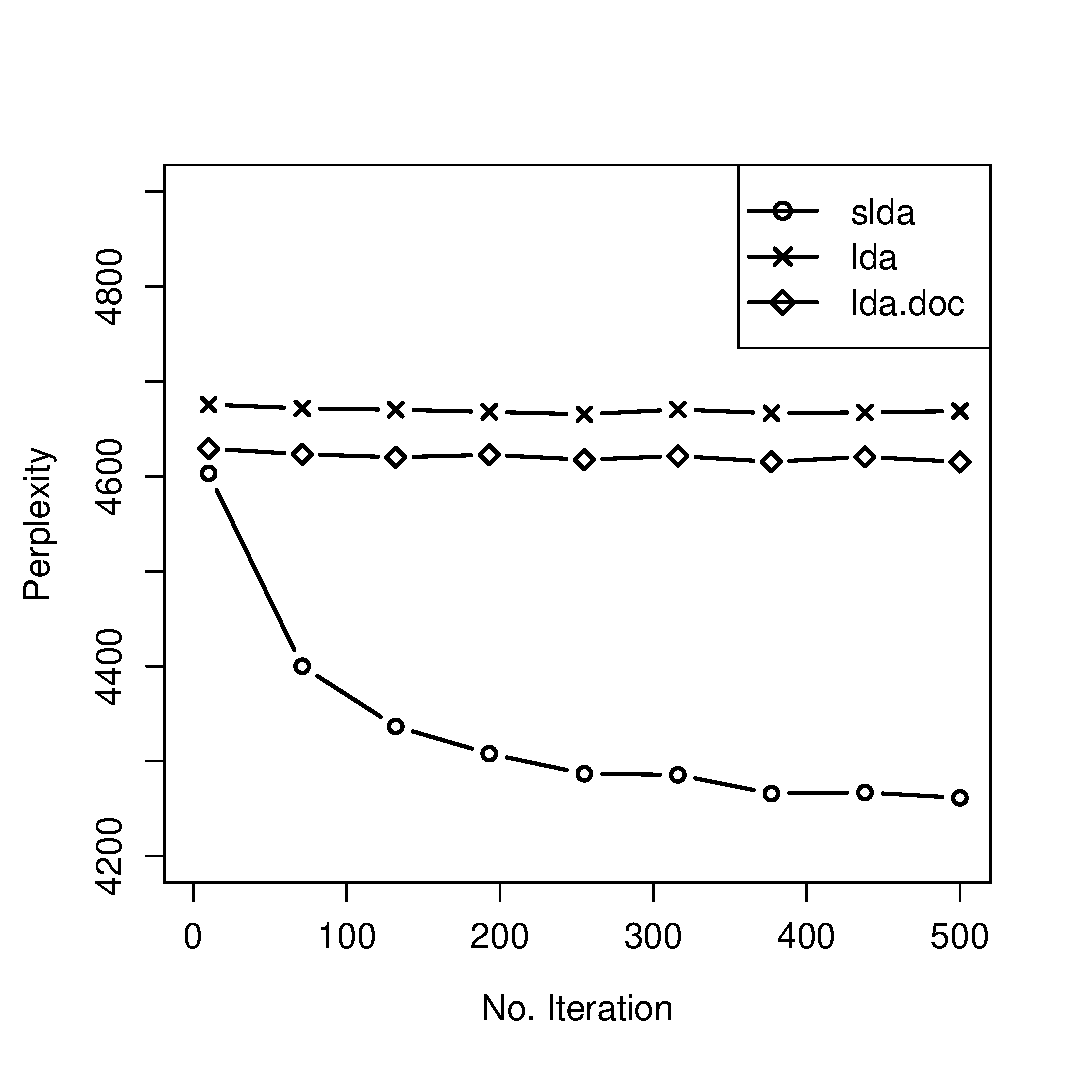
\includegraphics[width=\columnwidth]{ppl.eps}
  \caption{Performance of the three topic models in terms of test-set
  perplexity on the Penn TreeBank.  The sentence-layered LDA is denoted as {\tt
  slda}, the original LDA trained on sentence level as {\tt lda}, and the
  original LDA trained on document level as {\tt lda.doc} }
  \label{f:perplexity}
\end{figure}

\section{Perplexity Evaluation} \label{s:perplexity-evaluation}

One way to assess the performance of a topic model is through test-set
perplexity.  Test-set perplexity measures how well the model generalizes on
a held-out data.  Perplexity is measured in the amount of uncertainty, which is
a positive real number.  The lower perplexity we achieve for the model, the better
fit the model is for the data.  Generally, the test perplexity is derived as:
%--------------------------------------------------
% \begin{eqnarray*} \mathrm{perplexity_{test}} &=& \exp(\frac{- \log
% \Pr(\mathbf{w}_\mathrm{test})}{N_\mathrm{test}}) \\ &=& \exp(\frac{- \sum_w
% \log \Pr(w|d_\mathrm{test})}{N_\mathrm{test}}) \end{eqnarray*}
%-------------------------------------------------- 
\[ \mathrm{perplexity_{test}} = \exp(\frac{- \sum_w \log \Pr(w|d_\mathrm{test})}{N_\mathrm{test}}) \]

The key is to formulate $\Pr(w_\mathrm{test})$ for different topic models.  For
LDA, the probability is evaluated as follows.  \[ \Pr(w|d_\mathrm{test}) =
\sum_z \Pr(w|z) \Pr(z|d) \] The probability for the sentence LDA is a
bit more complicated due to an additional layer of latent semantics.  \[
\Pr(w|d_\mathrm{test}) = \sum_x \sum_z \Pr(w|z) \Pr(z|x) \Pr(x|d) \]
To infer all these probabilities, we loaded the trained model back in for
initializing $\Pr(w|z)$ in both model.  Since the training and the test sets do
not actually share documents and sentences, the rest of the probabilities
related to $z$, $x$, and $d$ need to be evaluated solely on the test data.  We
employed the same Gibbs sampling procedure with the preloaded counts for
$\Pr(w|z)$ and started another 500-iteration burn-in on the test sets.  For
simplicity, we read out only one sample for $\Pr(z|x)$ and $\Pr(x|d)$ at the
end of burn-in (and did the same thing for $\Pr(z|d)$ in the LDA model).

The Penn TreeBank is composed of 2,312 parsed documents, where each document
contains 21.2837 sentences in average.  We further divided the TreeBank into
two sets, one of 2,300 documents and the other of 154.  We trained the topic
models on the first set and evaluated the perplexities on the second.  For both
model, we had the Gibbs sampler burned in for 1,000 iterations before reading
out probabilistic estimates.  The number of word topics $T$ for both models are
set to be 10, as we figured the word topics in both models are functionally
equivalent and therefore they should be set to the same value.  The number
sentence topics for the sentence-layered model, however, were assigned to a
empirical value 20 that generally achieved best performance in our own tests.
We believed that such type of arrangement works
best in this comparative study. 

We had the parameters of the LDA model set up as suggested in
\cite{griffiths2004finding}, i.e., $\alpha = 50 / T$ and $\beta = 0.01$.  For
the sentence-layered LDA, the parameter is determined by applying the
regression result described in Section~\ref{s:parameter-estimation}.  In this
experiment, we tested three type of topic models: sentence-layered LDA, and two
LDA runs separately trained on the document level and the sentence level.  When
trained on the document level, LDA discard sentence boundary and treat the
entire document as one text unit; while on the sentence level, LDA treat each
sentence as individual ``documents''.  Tests were done only at the sentence
level.  

The experimental result showed that our approach achieved even lower test-set
perplexity than the other two LDA runs did.  As shown in
Figure~\ref{f:perplexity}, the perplexity for our model got convergence in
roughly 300 iterations; while those for the LDA models grew stable in a fairly
early stage.  We figured that both LDA models suffered from the following two
issues.  First, when the LDA model working in the sentence level, the
association of topic words did not go across the sentence boundaries, and thus
resulted in a loss of co-occurrence statistics.  Second, the LDA model trained
on the documents disregarded the syntax structures and treated all the word
occurrences as equally important; as a result, the model overfitted the data
and failed to address the diversity of co-occurred words in sentence level.  It
turned out employing a mixture of multiple sentence-layered LDA mitigate the
problems without much burden and best interpreted the word distribution for the
test data.

%--------------------------------------------------
% \subsection{Topic Examples} \label{ss:topic-examples}
% 
% \comment{ (Half a page) Here we briefly describe the word topics and show some example cluster }
% 
% \begin{table*}[!ht]
%   \footnotesize
%   \begin{tabular}{llllllllll}
% 
% bush & 0.006447 & million & 0.045660 & market & 0.020823 & president & 0.014135 & company & 0.009599\\
% federal & 0.006197 & year & 0.020008 & stock & 0.010724 & chief & 0.009355 & million & 0.008671\\
% court & 0.005780 & share & 0.018079 & trading & 0.008483 & executive & 0.008839 & new & 0.006577\\
% president & 0.005502 & billion & 0.013913 & investors & 0.007897 & vice & 0.007051 & year & 0.004713\\
% house & 0.005058 & quarter & 0.013669 & more & 0.006490 & company & 0.006948 & billion & 0.004699\\
% judge & 0.004891 & company & 0.013540 & stocks & 0.006125 & officer & 0.006191 & corp & 0.004303\\
% rrb & 0.004502 & cents & 0.009978 & prices & 0.005929 & chairman & 0.005881 & more & 0.004282\\
% state & 0.004474 & shares & 0.008423 & big & 0.005369 & sales & 0.005503 & inc & 0.004210\\
% white & 0.004363 & sales & 0.008333 & program & 0.004991 & corp & 0.005159 & out & 0.003958\\
% lrb & 0.004280 & net & 0.008037 & traders & 0.004717 & damage & 0.005056 & bank & 0.003720\\
% congress & 0.004169 & corp & 0.007484 & markets & 0.004652 & san & 0.004644 & group & 0.003505\\
% case & 0.003863 & third & 0.007471 & price & 0.004496 & named & 0.004609 & two & 0.003310\\
% committee & 0.003835 & earlier & 0.007330 & money & 0.004300 & francisco & 0.004609 & last & 0.003289\\
% bill & 0.003752 & rose & 0.006815 & futures & 0.004287 & products & 0.004334 & under & 0.003267\\
% against & 0.003668 & earnings & 0.006507 & many & 0.004105 & inc & 0.004300 & buy & 0.003238\\
% senate & 0.003502 & inc & 0.006365 & index & 0.003753 & rnr & 0.003990 & years & 0.003159\\
% law & 0.003224 & stock & 0.005838 & new & 0.003753 & director & 0.003784 & business & 0.003030\\
% political & 0.003196 & revenue & 0.005414 & buy & 0.003571 & area & 0.003543 & one & 0.002986\\
% government & 0.003196 & new & 0.005349 & funds & 0.003558 & ibm & 0.003406 & tax & 0.002943\\
% east & 0.003141 & profit & 0.005272 & companies & 0.003401 & new & 0.003165 & first & 0.002943\\
% \hline
% new & 0.008341 & cancer & 0.005641 & out & 0.004540 & year & 0.012195 & plant & 0.007408\\
% one & 0.007973 & drug & 0.004275 & san & 0.003982 & stock & 0.011907 & corp & 0.005953\\
% more & 0.006784 & health & 0.003741 & one & 0.003982 & new & 0.009746 & plants & 0.004102\\
% people & 0.004897 & university & 0.003385 & more & 0.003266 & trading & 0.009722 & company & 0.003970\\
% years & 0.004708 & gene & 0.002910 & francisco & 0.003226 & index & 0.008738 & china & 0.003903\\
% out & 0.004444 & cbs & 0.002910 & air & 0.002907 & shares & 0.007874 & more & 0.003903\\
% now & 0.004416 & human & 0.002792 & earthquake & 0.002907 & market & 0.007562 & magazine & 0.003771\\
% time & 0.004189 & institute & 0.002495 & steel & 0.002907 & average & 0.007346 & products & 0.003110\\
% such & 0.003963 & noriega & 0.002257 & three & 0.002469 & down & 0.007010 & cars & 0.002912\\
% two & 0.003803 & course & 0.002257 & market & 0.002469 & prices & 0.006914 & 000 & 0.002647\\
% year & 0.003680 & team & 0.002257 & equipment & 0.002390 & york & 0.006866 & drug & 0.002581\\
% ich & 0.003680 & sports & 0.002198 & city & 0.002270 & exchange & 0.006818 & build & 0.002449\\
% many & 0.003425 & patients & 0.002198 & corp & 0.002191 & rate & 0.006794 & air & 0.002449\\
% lrb & 0.003369 & researchers & 0.002139 & over & 0.002151 & month & 0.006578 & auto & 0.002383\\
% over & 0.003284 & heat & 0.002139 & home & 0.002032 & days & 0.005930 & production & 0.002383\\
% rrb & 0.003255 & football & 0.002079 & system & 0.002032 & yen & 0.005570 & producers & 0.002316\\
% 000 & 0.003170 & genes & 0.001901 & game & 0.002032 & points & 0.005498 & egg & 0.002250\\
% business & 0.003161 & man & 0.001782 & service & 0.001952 & rose & 0.005402 & equipment & 0.002250\\
% american & 0.003095 & jones & 0.001782 & stores & 0.001952 & fell & 0.005330 & japan & 0.002250\\
% even & 0.003001 & white & 0.001782 & computer & 0.001912 & billion & 0.005306 & world & 0.002184\\
%   \end{tabular}
%   \caption{Topic clusters for sentence-layered LDA trained on the Penn TreeBank.}
%   \label{t:topic-cluster-slda}
% \end{table*}
% 
% \begin{table*}[!ht]
%   \footnotesize
%   \begin{tabular}{llllllllll}
% 
% out & 0.025053 & bank & 0.016592 & rrb & 0.024270 & corp & 0.028034 & prices & 0.016212\\
% time & 0.018857 & securities & 0.014099 & lrb & 0.023996 & inc & 0.020579 & interest & 0.014718\\
% many & 0.017699 & bonds & 0.013166 & before & 0.011998 & company & 0.018514 & rate & 0.013060\\
% more & 0.017646 & investment & 0.012628 & house & 0.011360 & companies & 0.016450 & analysts & 0.010783\\
% even & 0.015028 & money & 0.012305 & under & 0.010831 & based & 0.012547 & much & 0.010638\\
% people & 0.014975 & through & 0.012018 & plan & 0.009974 & industry & 0.011812 & long & 0.010383\\
% still & 0.012090 & capital & 0.011426 & ich & 0.008133 & unit & 0.010447 & japanese & 0.010182\\
% those & 0.011538 & issue & 0.009435 & law & 0.007786 & products & 0.009765 & rates & 0.010182\\
% now & 0.010274 & debt & 0.009417 & bill & 0.007458 & international & 0.008855 & recent & 0.009490\\
% such & 0.009776 & funds & 0.009346 & one & 0.007075 & including & 0.008242 & higher & 0.009217\\
% way & 0.007870 & offer & 0.009184 & city & 0.007039 & computer & 0.008242 & expected & 0.009017\\
% good & 0.007692 & part & 0.009112 & case & 0.006710 & operations & 0.007927 & trade & 0.008998\\
% small & 0.007443 & yield & 0.008521 & congress & 0.006692 & group & 0.007682 & major & 0.008670\\
% far & 0.006535 & bond & 0.008485 & line & 0.005835 & oil & 0.007385 & lower & 0.008543\\
% news & 0.006499 & each & 0.008449 & white & 0.005762 & used & 0.006982 & foreign & 0.008434\\
% number & 0.006482 & sold & 0.007947 & set & 0.005744 & national & 0.006772 & high & 0.008288\\
% little & 0.006357 & banks & 0.007857 & whether & 0.005580 & concern & 0.006755 & growth & 0.008124\\
% think & 0.006339 & common & 0.007821 & policy & 0.005470 & services & 0.006650 & term & 0.007942\\
% same & 0.006250 & pay & 0.007713 & committee & 0.005306 & contract & 0.006422 & economic & 0.007924\\
% though & 0.006019 & cash & 0.007552 & judge & 0.005033 & service & 0.006335 & japan & 0.007887\\
% \hline
% million & 0.087200 & two & 0.026314 & new & 0.054527 & president & 0.024608 & government & 0.017090\\
% year & 0.059195 & one & 0.026204 & market & 0.044860 & business & 0.021042 & federal & 0.016910\\
% billion & 0.035402 & years & 0.024279 & stock & 0.037836 & company & 0.015519 & state & 0.013338\\
% share & 0.032287 & more & 0.022885 & trading & 0.024692 & financial & 0.013006 & officials & 0.010825\\
% 000 & 0.023358 & over & 0.020629 & shares & 0.024053 & chairman & 0.012821 & against & 0.009873\\
% quarter & 0.021983 & three & 0.015458 & york & 0.019512 & american & 0.012711 & such & 0.009694\\
% sales & 0.021374 & week & 0.014780 & exchange & 0.016550 & chief & 0.012193 & court & 0.008706\\
% company & 0.016935 & month & 0.013661 & price & 0.016230 & executive & 0.012138 & department & 0.008006\\
% first & 0.016361 & ich & 0.013478 & yesterday & 0.015113 & well & 0.010604 & insurance & 0.007629\\
% cents & 0.015839 & next & 0.013185 & down & 0.014173 & both & 0.010013 & public & 0.007396\\
% earlier & 0.014725 & last & 0.012855 & big & 0.014120 & firm & 0.009884 & bush & 0.007181\\
% rose & 0.013942 & days & 0.010526 & stocks & 0.012949 & make & 0.009515 & use & 0.007163\\
% third & 0.013541 & world & 0.010269 & board & 0.012612 & take & 0.009016 & office & 0.007037\\
% net & 0.012636 & between & 0.009774 & index & 0.011867 & management & 0.008665 & tax & 0.006768\\
% earnings & 0.012497 & during & 0.009499 & program & 0.011743 & work & 0.008406 & california & 0.006516\\
% last & 0.011592 & old & 0.009169 & investors & 0.010980 & exp & 0.008388 & help & 0.006122\\
% profit & 0.010565 & five & 0.009022 & day & 0.010909 & vice & 0.008295 & without & 0.005745\\
% income & 0.010287 & another & 0.008417 & average & 0.009472 & very & 0.007704 & administration & 0.005637\\
% revenue & 0.009173 & plans & 0.008142 & friday & 0.009064 & rnr & 0.007353 & made & 0.005583\\
% loss & 0.008337 & past & 0.008142 & buy & 0.008816 & director & 0.007187 & life & 0.005565\\
% 
%   \end{tabular}
%   \caption{Topic clusters for the original LDA (sentence level) trained on the Penn TreeBank.}
%   \label{t:topic-cluster-lda}
% \end{table*}
% 
% As a result of the previous experiment, we fetched the top-20 most
% representative words from the topic clusters for both the LDA and
% sentence-layered models.  The snapshots are shown in
% Tables~\ref{t:topic-cluster-slda} and \ref{t:topic-cluster-lda}, respectively.
% 
% \comment{NOTE: We cannot afford put two big tables here.  Select two or three
% comparable clusters from both model as an example.}
%-------------------------------------------------- 

%--------------------------------------------------
% \comment{FIX IT: Add the results on ACL abstracts.}
%-------------------------------------------------- 

%--------------------------------------------------
% \subsection{Cohesion Test}
% 
% { \color{red} NOTE: This task is proposed in replace of the haystack evaluation. }
% { \color{red} (Page 6, half a page) Describe the idea of the cohesion test. }
% 
% The cohesion test is another way for evaluating how well a probabilistic model
% generalizes the data.  We assume that, a probabilistic model should be able to
% tell how coherent the content of a document is by looking at the query
% likelihood, which is functionally equivalent to the test-set perplexity.  We
% expect that a coherent document results in a lower perplexity while an
% incoherent document a higher one.  
% 
% One way to form an incoherent set of document is through sentence ``swap-in''.
% Given a document $d$ and a set of sentences ${ s_1, s_2, \ldots, s_N }$
% (candidates) drawn from the test data, we randomly chose one sentence (some $q
% \in d$) from the document and replace it with any sentence from the candidate
% set.  By repeating the last step $N$ times, we form a synthesis document set.
% Now, we present the original document $d$ together with the synthesis set and
% asked the model to sort the documents in the order of test-set perplexity.  We
% look at the rank the original document is positioned in each run and evaluate
% the model performance by mean-reciprocal rank.  In this task, we still used
% Penn TreeBank as our test corpora.  The result is shown in the following
% section ({\color{red} FIX IT}).
%-------------------------------------------------- 

%--------------------------------------------------
% \subsection{``Haystack'' Task}
% 
% { \color{red} NOTE: This evaluation is no longer useful in this work.  Might be
% removed anytime soon. }
% 
% { \color{red} (Page 6, half page) Describe the idea of doing haystack task. 
% 
% The ``hay'' sentences groups come from the Multiple-Translation Chinese Corpus
% Part 1 to Part 4.  The ``stack'' corpus that we used in this experiment is the
% Xinhua News Service (XIE) from the English Gigaword, which contains 4,517,671
% sentences in totally 679,007 documents.  For convenience we further break down
% the corpus into 12 folds.  The performance is measured by top-k accuracy and
% mean reciprocal rank.  Participants include 1) tf-idf, 2) unigram (bi-gram)
% language model, 3) LDA, and 4) Sentence LDA + bigram.  The tf-idf model doesn't
% have parameters for us to fine-tune. }
%-------------------------------------------------- 


%--------------------------------------------------
% Other stuff
%-------------------------------------------------- 
\section{Related Work} \label{s:related-work} 

Our work was inspired by a number of efforts for extending the LDA model,
including Pachinko allocation model \cite{li2006pachinko}, nested Chinese
restaurant process \cite{blei2004hierarchical}, and mixture network
\cite{heinrich2009generic}.  Among other efforts that we have gradually learned
about during the development of this work, the most similar to our approach is
the latent-Dirichlet co-clustering model \cite{shafiei2006latent}.  While the
previous research went through complicated formulation in light of modeling the
correlation between topics, our preliminary study for LDA mixture made in the
sentence level tried to bridge the gap between the document and the words.  Our
proposed model can be seen as a specialization of these efforts all together
for improving the model interpretability at a finer scale.

\section{Discussions} \label{s:discussions} 
While the LDA has been proven quite successful in discovery task for word
topics, one drawback of the model remains its inability to offer fine-grain
topic distribution, being unprecise to sample the document-level multinomial.
Our model, being one of the descendents of LDA, is likely to inherit this flaw.
Our expectation to simultaneously improve word-cluster and document-cluster
precision did not come true.  Through experimentation, we showed that, by
offering enough number of sentence-level mixtures, the layered model can better
fit the underlying data, resulting in better probability estimate for the
generation of word topics.  However, it remains rather difficult for us to put
the topic distribution to direct use.  

Far as we have learned, certain applications that a precise topic distribution
can benefit have already seen indirect use of the topic models, and most of
these effort heavily relied on the rich topic features provided by inspecting
word clusters.  A direct application of the topic distribution might be more
appealing either in theoretical or practical point of view.  Our preliminary
study on integrating a layered mixture of multinomials is only an early step
toward this big challenge.

\newpage
%--------------------------------------------------
% \section*{Acknowledgements}  We thank Kenji Sagae for useful discussions.  The
% project or effort describe here has been sponsored by the U.S. Army Research,
% Development, and Engineering Command (RDECOM).  Statements and opinions
% expressed do not necessarily reflect the position or the policy of the United
% States Government, and no official endorsement should be inferred.
%-------------------------------------------------- 
